\documentclass[tikz]{standalone}
\usetikzlibrary{shapes, arrows.meta}

\begin{document}
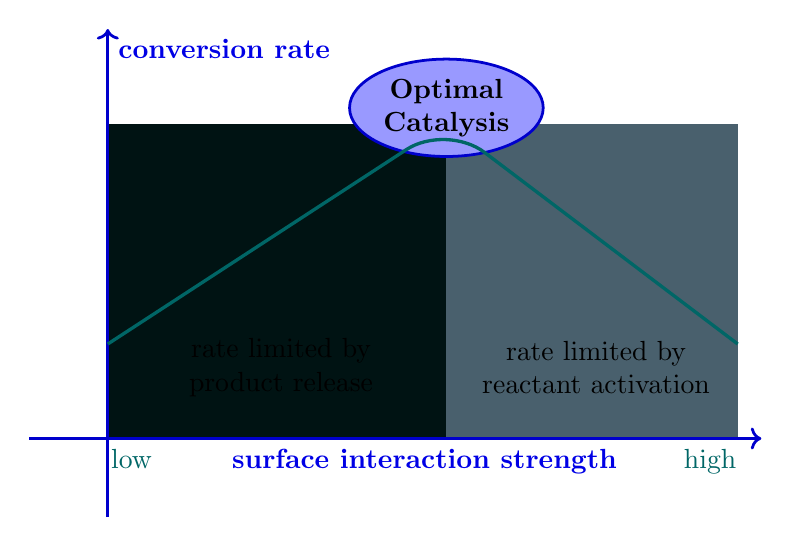
\begin{tikzpicture}[thick, align=center]

  % Foreground regions with new colors
  \fill[teal!15!black] (0,0) rectangle (4.3,4);
  \fill[cyan!35!black] (4.3,0) rectangle (8,4);

  % Chemistry domain node labels
  \node at (2.2,0.9) {rate limited by\\product release};
  \node at (6.2,0.9) {rate limited by\\reactant activation};
  \node[ellipse, draw=blue!80!black, fill=blue!40!white, line width=1pt, inner sep=2pt, font=\bfseries] at (4.3,4.2) {Optimal\\Catalysis};

  % Axes
  \draw[->, line width=1pt, color=blue!80!black] (-1,0) -- (8.3,0)
    node[below, pos=0.14, color=teal!80!black] {low}
    node[below, pos=0.54, font=\bfseries, color=blue!90!black] {surface interaction strength}
    node[below, pos=0.93, color=teal!80!black] {high};
  \draw[->, line width=1pt, color=blue!80!black] (0,-1) -- (0,5.2)
    node[below right, font=\bfseries, color=blue!90!black] {conversion rate};

  % Line-graph curve (updated equation shape)
  \draw[rounded corners=4ex, very thick, color=teal!80!black]
    (0,1.2) -- (4.3,4) -- (8,1.2);

\end{tikzpicture}
\end{document}